\chapter{Описание принципа работы подсистемы Ethernet}
\section{Разъем RJ-25, трансформатор и обвязка}
\hspace{1cm} 

Рассмотрим основные особенности, связанные с связанные со схемотехникой Ethernet части. 

На рисунке \ref{ris:RJ-45} изображена часть подсистемы от разъема RJ-45 до согласующего трансформатора. 

\begin{figure}[H]
\centering
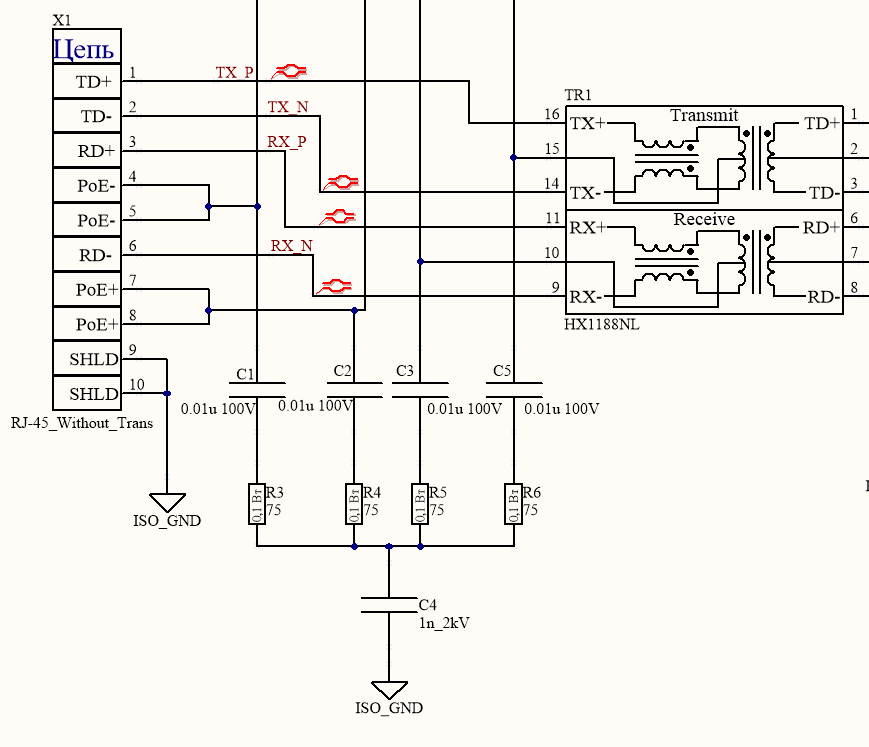
\includegraphics[scale = 0.6]{RJ-45_Bob_Smith.png}
\caption{Часть подсистемы Ethernet от разъема RJ-45 до согласующего трансформатора}
\label{ris:RJ-45}
\end{figure}

Здесь линии TD+, TD- и RD+, RD- попарно представляют собой линии передачи и приема информации через Ethernet. 
конструктивно они реализуются в виде дифференциальных пар. 
Идея дифференциальной передачи сигналов проста. Вместо передачи одного
сигнала передаются два. Одновременно с полезным сигналом передается второй
сигнал, точно такой же, как первый сигнал, но противоположной полярности.
Возвратный ток первого сигнала — положительный. Возвратный ток второго сигнала — 
отрицательный. Они нейтрализуют друг друга \ref{ris:DiffPair}

\begin{figure}[H]
\centering
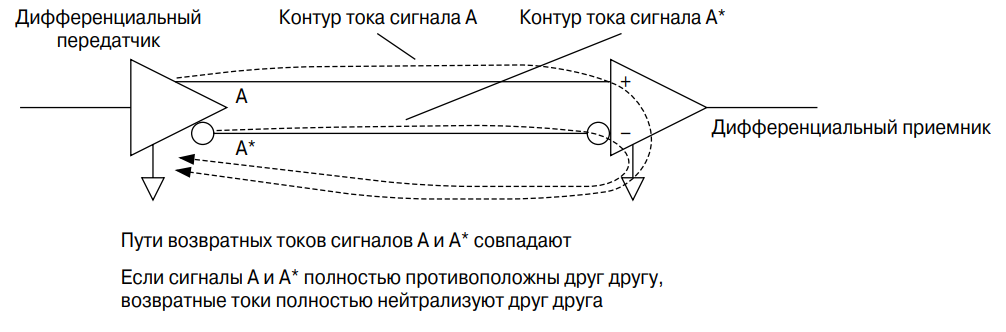
\includegraphics[scale = 0.65]{DiffPair.png}
\caption{Дифференциальная передача сигнала обеспечивает взаимную нейтрализацию
возвратных токов}
\label{ris:DiffPair}
\end{figure}

В приемнике производится сравнение двух сигналов для определения полярности логических сигналов. Для 
выполнения операции сравнения в приемнике нетребуется внутреннего опорного напряжения. Напряжения сдвига земли
между передатчиком и приемником оказывают одинаковое воздействие на режим работы
обеих линий передачи, поэтому не влияют на разность сигналов, передаваемых по ним. 
Режим приема дифференциального сигнала не подвержен влиянию напряжения сдвига земли между передатчиком и 
приемником.

В случае дифференциального сигнала единственной причиной появления возвратного тока в цепи передачи является 
разбаланс сигналов дифференциальной пары. Если сигналы дифференциальной пары не идеально противоположны друг
другу, то полной взаимной нейтрализации возвратных токов сигналов не происходит. Этот ток разбаланса называется 
синфазным током. У качественного дифференциального передатчика синфазный ток в 100 раз меньше тока полезного
сигнала. Снижение синфазного тока обеспечивает снижение уровня электромагнитного излучения 
\cite{Howard J: Start Black Magic}.

Для граммотной трассировки этих линий, нужно расчитать их ширину, с учетом конструктивных особенностей 
платы, для соблюдения необходиммого импеданса, чтобы данные передавались корректно. 

Для расчета воспользуемся средствами Saturn PCB Toolkit V7.03. Согласно документации на PHY-микросхему,
целевой импеданс Ethernet линий должен быть равен 100 Ом \cite{DP83848:datasheet}. В качестве допуска 
возьмем 10\% от целевого импеданса. 

Результаты расчета представлены на рисунке \ref{ris:Saturn}

\begin{figure}[H]
\centering
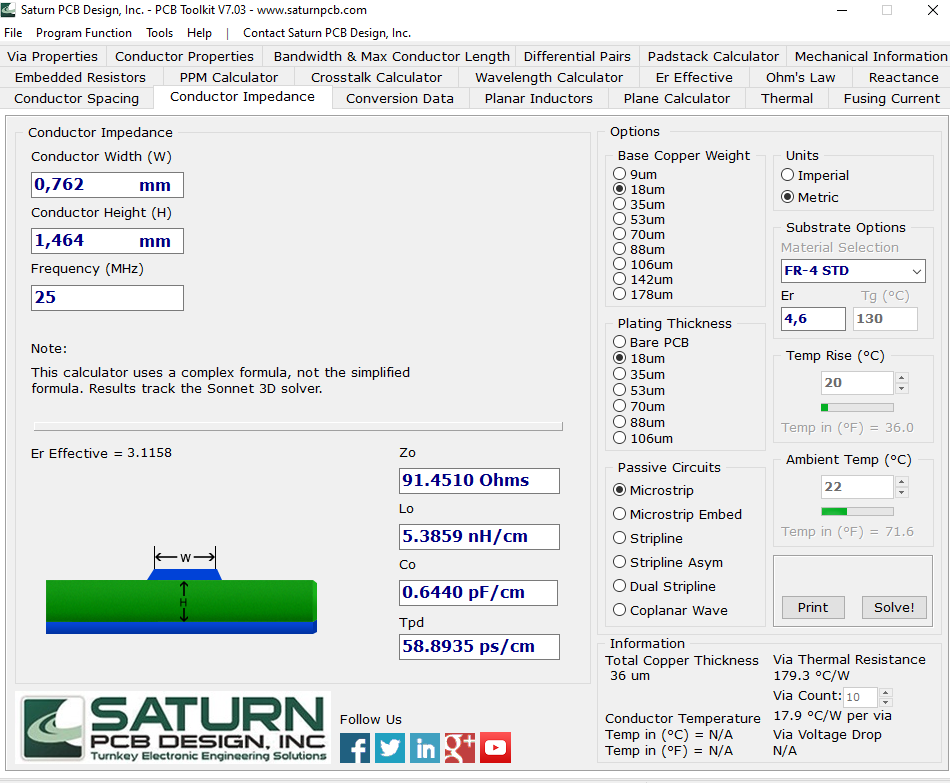
\includegraphics[scale = 0.65]{Saturn.png}
\caption{Результаты расчета импеданса линий передачи данных Ethernet в Saturn Toolkit}
\label{ris:Saturn}
\end{figure}

 Весь ход расчета определяет стек платы. Мы будем использовать стандартный стек компании ООО "Резонит". 
 Плата будет двуслойная, с толщиной фольги 18 мкм, общей толщиной 1,5 мм и, следовательно, толщиной 
 диэлектрика FR4 (Tg135) 1,464 мм. 

 В разделе <<Option>> задаем конструктивные особенности платы, выбираем материал диэлектрика, его 
 диэлектрическую проницаемость, конструктивное исполнение линий. 

 Далее в <<Conductor Impedance>> задаем толщину диэлектрика и максимальную тактовую частоту платы. Теперь 
 плавно меняя значение в поле <<Conductor Width>> пытаемся добиться целевого импеданса с заданной точностью. 

 Получившиеся значения устраиваемого нас импеданса представлены на рисунке \ref{ris:Saturn}. 
 
На рисунке \ref{ris:RJ-45} конденсаторы C1-C5 и резисторы R3-R6 образуют так называемый <<Bob Smith Terminations>>. 
Их использование дает нам следующие преимущества \cite{Bob Smith terminator}:

\begin{enumerate}
    \item Уменьшение шума отражения сигнала.
    \item Улучшение времени нарастания фронтов импульса снижая уровень электромагнитных помех 
    и обеспечивая дополнительный запас по времени.
    \item Из-за уменьшения отражений мы можем увеличить длину проводиммых дорожек, что облегчает трасировку.
    \item Резистивная нагрузка улучшает соотношение сигнал/шум.
\end{enumerate}

Далее рассмотрим рисунок \ref{PhyScheme}, на котором изображено соедниение между согласущим трансформатором 
и PHY-микросхемы DP83848, а так же обвязка ее и интерфейс RMII, соединющий DP83848 и микронтроллер. 

\begin{figure}[H]
\centering
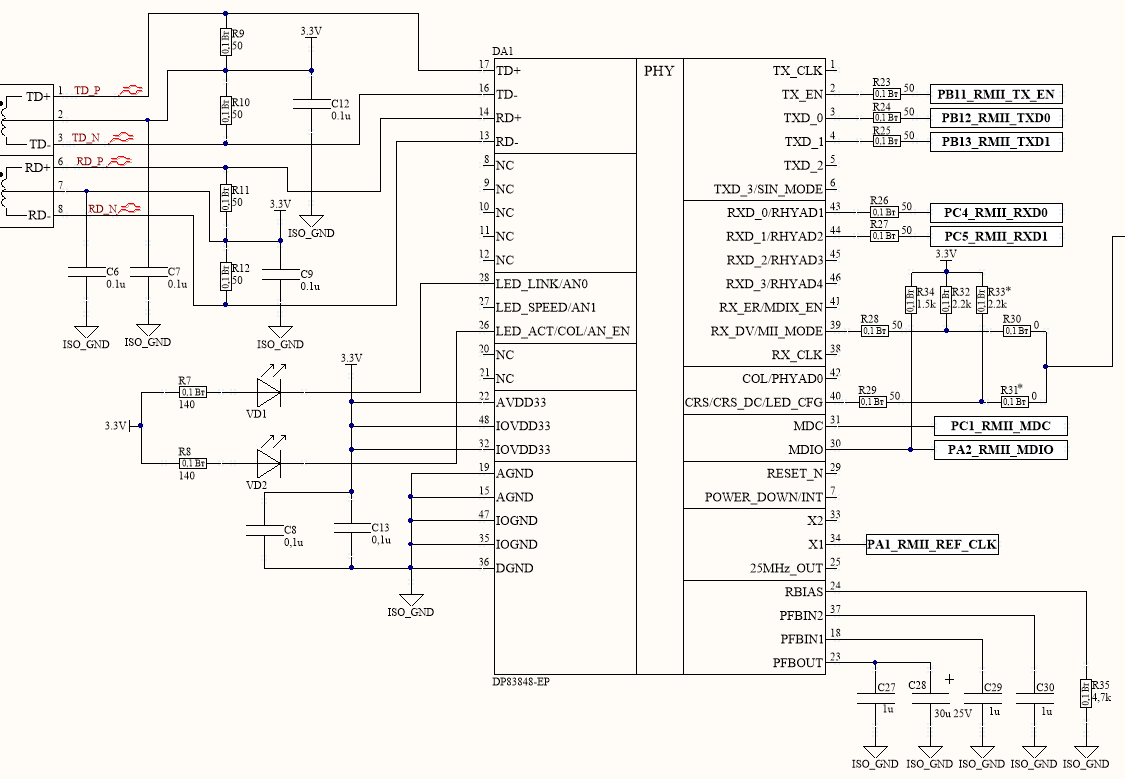
\includegraphics[scale = 0.6]{PHY scheme.png}
\caption{Результаты расчета импеданса линий передачи данных Ethernet в Saturn Toolkit}
\label{ris:Saturn}
\end{figure}

Резисторы R9-R12 являются согласующими для линий дифференциальной передачи, их номинал равен 50 Ом и топологически 
их следует распологать как можно ближе к PHY-микросхеме, реализуя согласование последовательным резистором на 
стороне приемника. 

